% Chapter 2

\chapter{Learning Bayesian Networks} % Main chapter title

\label{Chapter2} % For referencing the chapter elsewhere, use \ref{Chapter1} 

\lhead{Chapter 2. \emph{Learning}} % This is for the header on each page - perhaps a shortened title
Bayesian networks are directed acyclic graphs (DAG). They are representations of the dependence structure among a set of random variables. The conditional dependencies between these random variables are visualized via directed edges and the random variables themselves are the nodes of the network. Through the directed edges it is possibly to identify a hierarchy. Nodes having edges leading to another node are called parents of the receiving node. Similarly, the receiving node is a child of the source node. Besides the dependence structure the nodes in a Bayesian Network carry a probability distribution conditional on their parents. In the case of discrete distributions this becomes a probability table.\\
The advantage of using a Bayesian Network is that it represents the joint probability over all the random variables considered. It is possible to answer conditional queries through the laws of probability theory. Through the structure of the network the joint probability distribution factorizes, leading to less parameters to be estimated and a more efficient computation.\\
For the task of the evaluation of natural hazard Bayesian Networks provide a consistent and efficient way to compute the full distribution of the target variable and thus to deal with the associated uncertainties.
\newpage

%----------------------------------------------------------------------------------------

\section{Choosing the Structure of Bayesian Networks}
The task for this assignment is to build different Bayesian Networks, use synthetic data to learn the corresponding parameters and evaluate their performance of predicting on the target value.\\
The data consists of a set of six variables commonly employed for defining ground motion models and the prediction of ground motion values. Each of the variables has been sampled from a distribution according to table~\ref{tab:Variables} and the stochastic model of~\cite{boore2003} was used to compute the corresponding values of PGA. In total the data set comprises 10.000 "observations". Since there is no simple analytic form of the stochastic model and it involves dealing with distributions from different families, the data has been discretized into intervals according to table~\ref{tab:discretization} and discrete Bayesian Networks are learned using multinomial distributions throughout.

\vspace{1cm}

\begin{table}[h]
\caption[Variables and Distributions]{Overview over the variables used and their according distributions.}
\begin{tabular}{ p{3cm}p{5cm}p{5cm}  }
\hline
 $X_i$ & Description & Distribution$_{[range]}$\\
 \hline 
 \hline
 \multicolumn{3}{c}{Variables} \\
 \hline
 M   & Moment Magnitude    &$\mathcal{U}_{[5,7.5]}$\\
 R&   Distance to Source  & Exp$_{[1 km, 200km]}$\\
 SD & Stress drop & Exp$_{[0 bar, 500bar]}$\\
 $Q_0$    &Attenuation of seismic waves in deep strata &  Exp$_{[0 s^{-1}, 5000 s^{-1}]}$\\
 $\kappa_0$&   Attenuation of seismic waves close to the surface  &  Exp$_{[0 s, 0.1 s]}$\\
 $V_s30$& Average shear wave velocity in the upper 30m  & $\mathcal{U}_{[600 m s^{-1}, 2800 m s^{-1}]}$\\
 \hline
 \multicolumn{3}{c}{Ground Motion Variable} \\
 \hline
 $\log PGA$& logarithm of peak horizontal ground acceleration  & synthetic calculated through the stochastic model of Boore \citep{boore2003}\\
 \hline
\end{tabular}
\label{tab:Variables}
\end{table}

\vspace{1cm}

\begin{table}[htb]
\caption[Discretization of the Variables]{Discretization of the Variables. The intervals have been chosen in order to minimize information loss.}
\begin{tabular}{l|c c c c c c c c c  }
Variable&   \multicolumn{9}{c}{Interval Borders}\\
\hline
SD&         0&  0.8792&   5.438&  14.92&       58&   500&      &      & \\
Q0&         0&     330&    5000&       &         &      &      &      & \\
$\kappa_0$& 0& 0.01053&  0.0345&    0.1&         &      &      &      & \\
$V_S30$&     600&  1704.5&    2800&       &         &      &      &      & \\
M&          5&   6.271&     7.5&       &         &      &      &      & \\
R&          1&    4.38& 15.4885&  55.84&      200&      &      &      & \\
log PGA& -Inf&  -5.135&  -3.722& -2.627& -1.20742& 0.145& 1.657& 3.175& Inf\\
\end{tabular}
\label{tab:discretization}
\end{table}

\newpage

\subsection{Naive Bayes Network}
There are different methods for choosing the structure of a Bayesian Network. The easiest and simplest way is to construct a Naive Bayes network. This means that the target value is connected to all explanatory values and there are no other dependencies. This is "naive" as it makes the assumption that all explanatory variables are independent from each other. Thus, the joint distribution factorizes simply to the following product:

\begin{center}
\small
P(PGA, SD, MAG, DIST, $Q_0, \kappa_0, V_s30$) = P(PGA)* P(SD$\mid$PGA)* \\P(MAG$\mid$PGA)*P(DIST$\mid$PGA)* P($Q_0\mid$PGA)* P($\kappa_0\mid$PGA)* P($V_s30\mid$PGA)\\
\normalsize
\end{center}

Considering the Naive Bayes independence assumption can be thought of the simplest model that can be created by using all variables. Neglecting all dependencies is a strong assumption which might result in an unrealistic model. Nevertheless, it is a attractive choice because it needs very few parameters to be estimated and it shows a reasonable performance in real-world applications such as email spam filter. It is also a good candidate as a starting point because it is questionable to build more complex models which perform worse. The network in figure~\ref{fig:naive} represents the Naive Bayes network for the given variables and was used in the further computations.

\begin{figure}[!htpb]
	\centering
		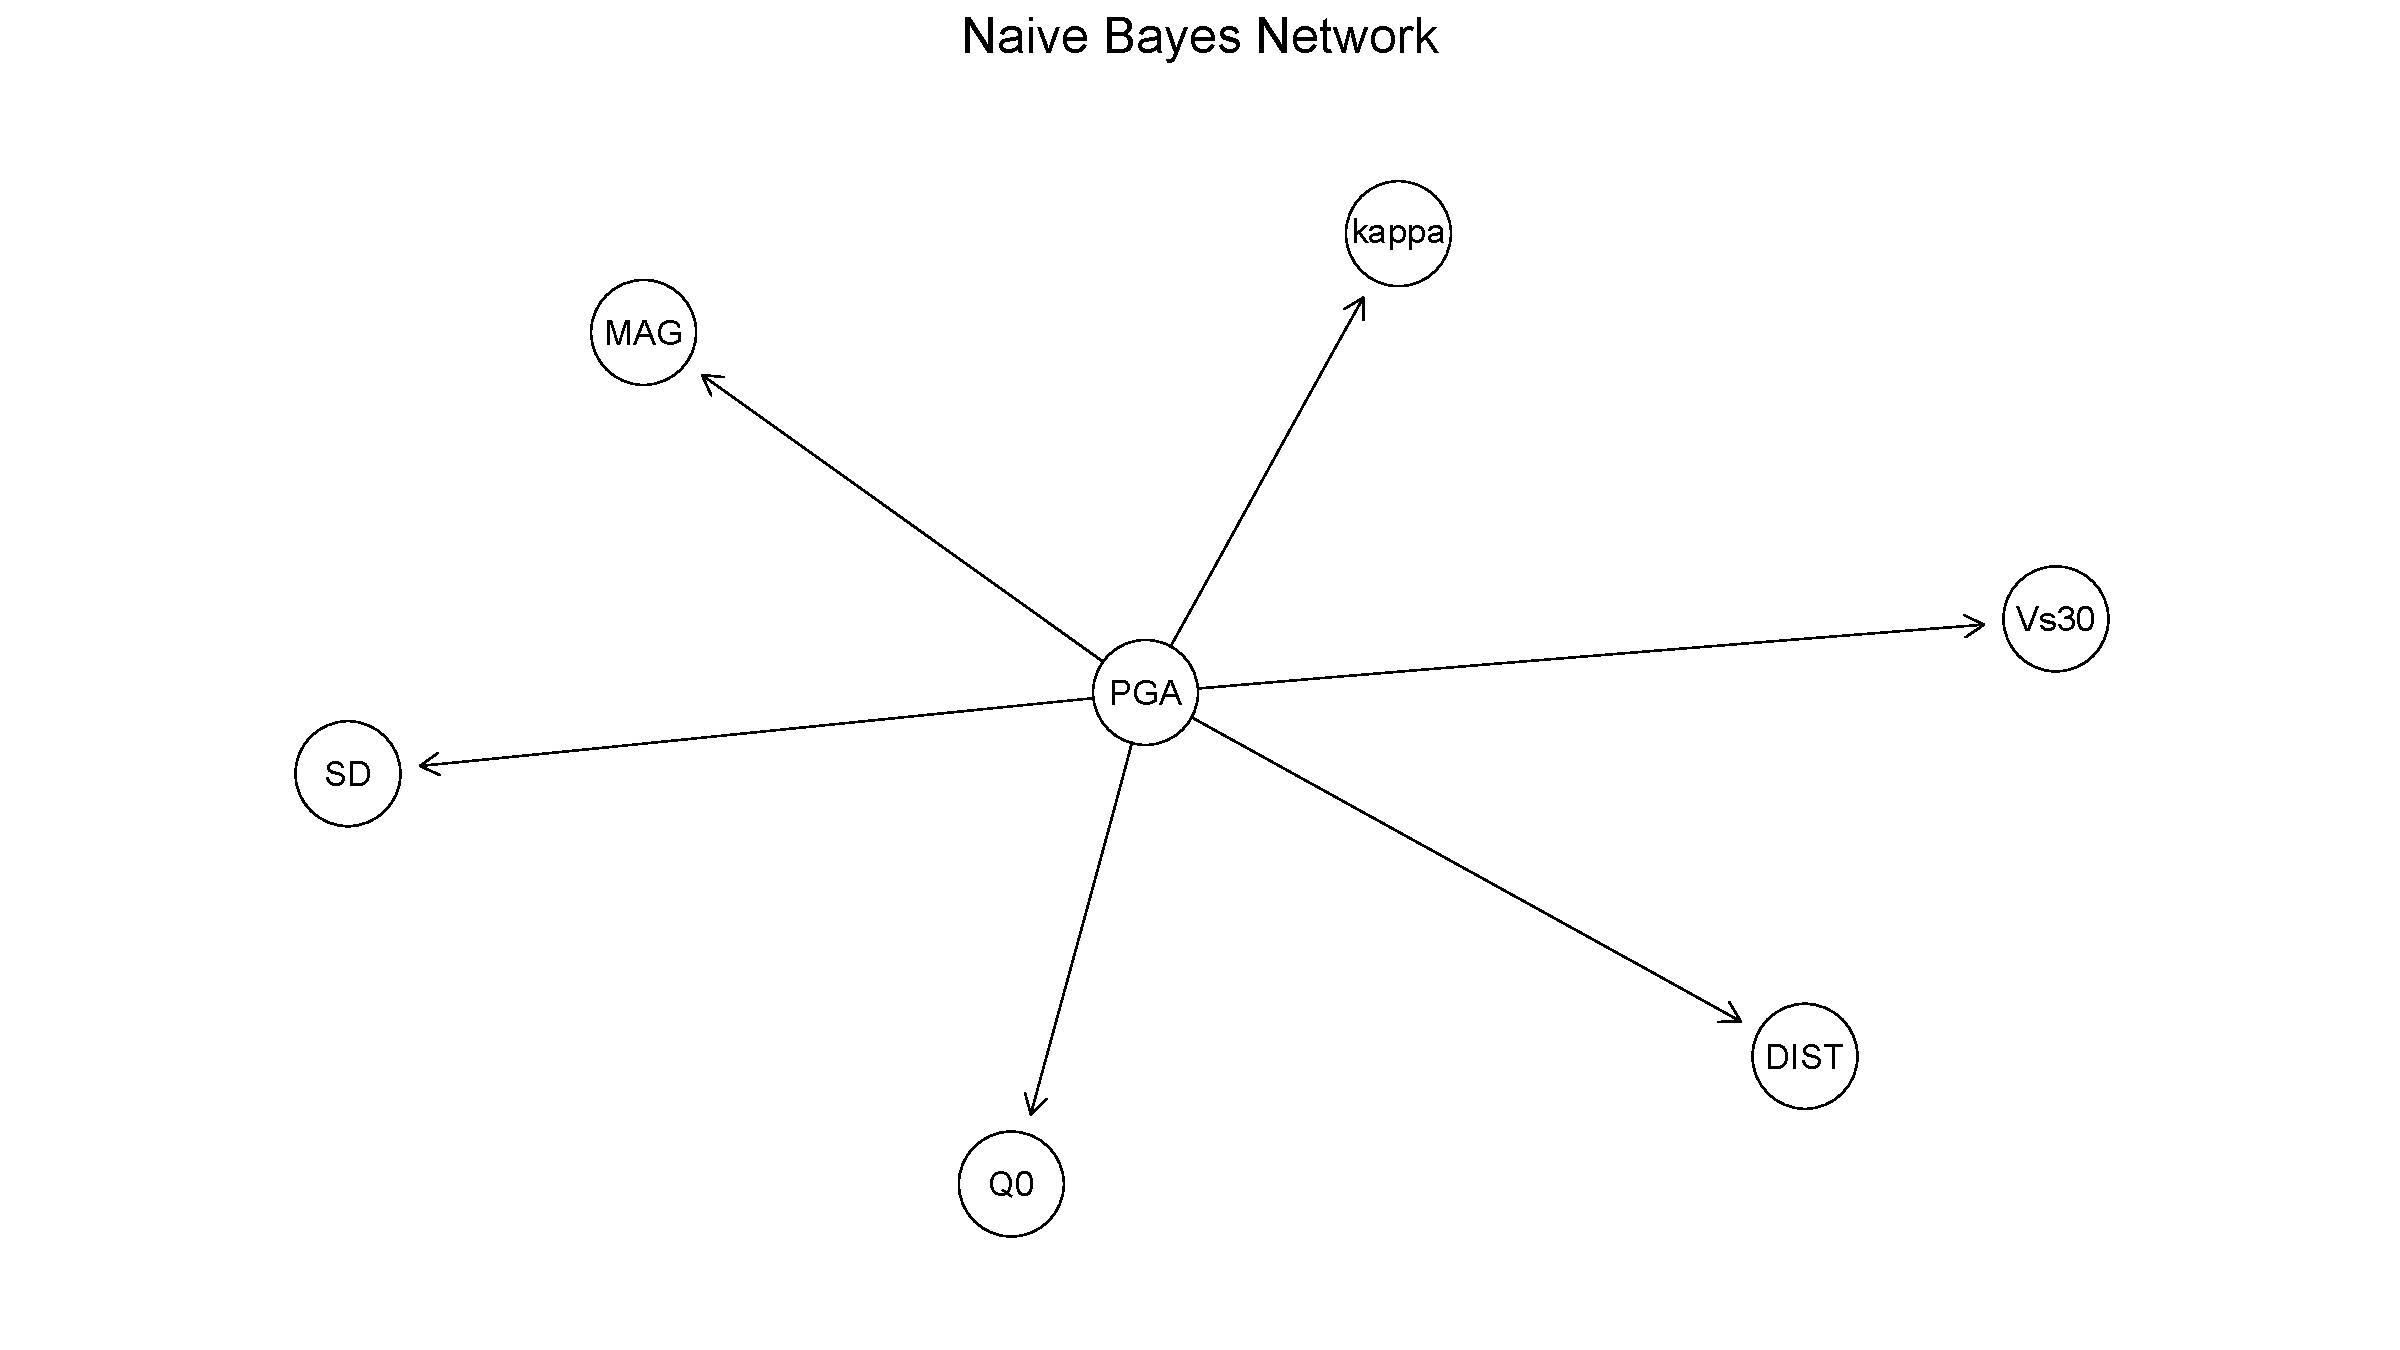
\includegraphics[scale=0.33]{Figures/naive.pdf}
		\rule{35em}{0.5pt}
	\caption[Naive Bayes Network]{The Naive Bayes network of the variables.}
	\label{fig:naive}
\end{figure}

\newpage

\subsection{Causal Network}

Another way of setting up the structure of a Bayesian Network is to rely on expert judgment to define the dependencies between the variables. This is called a causal network since one tries to capture the causal relationships among the variables. For the case of predicting PGA from a set of explanatory variables the following causal network (Figure~\ref{fig:causal}) can be reasoned.\\

\begin{figure}[!h]
	\centering
		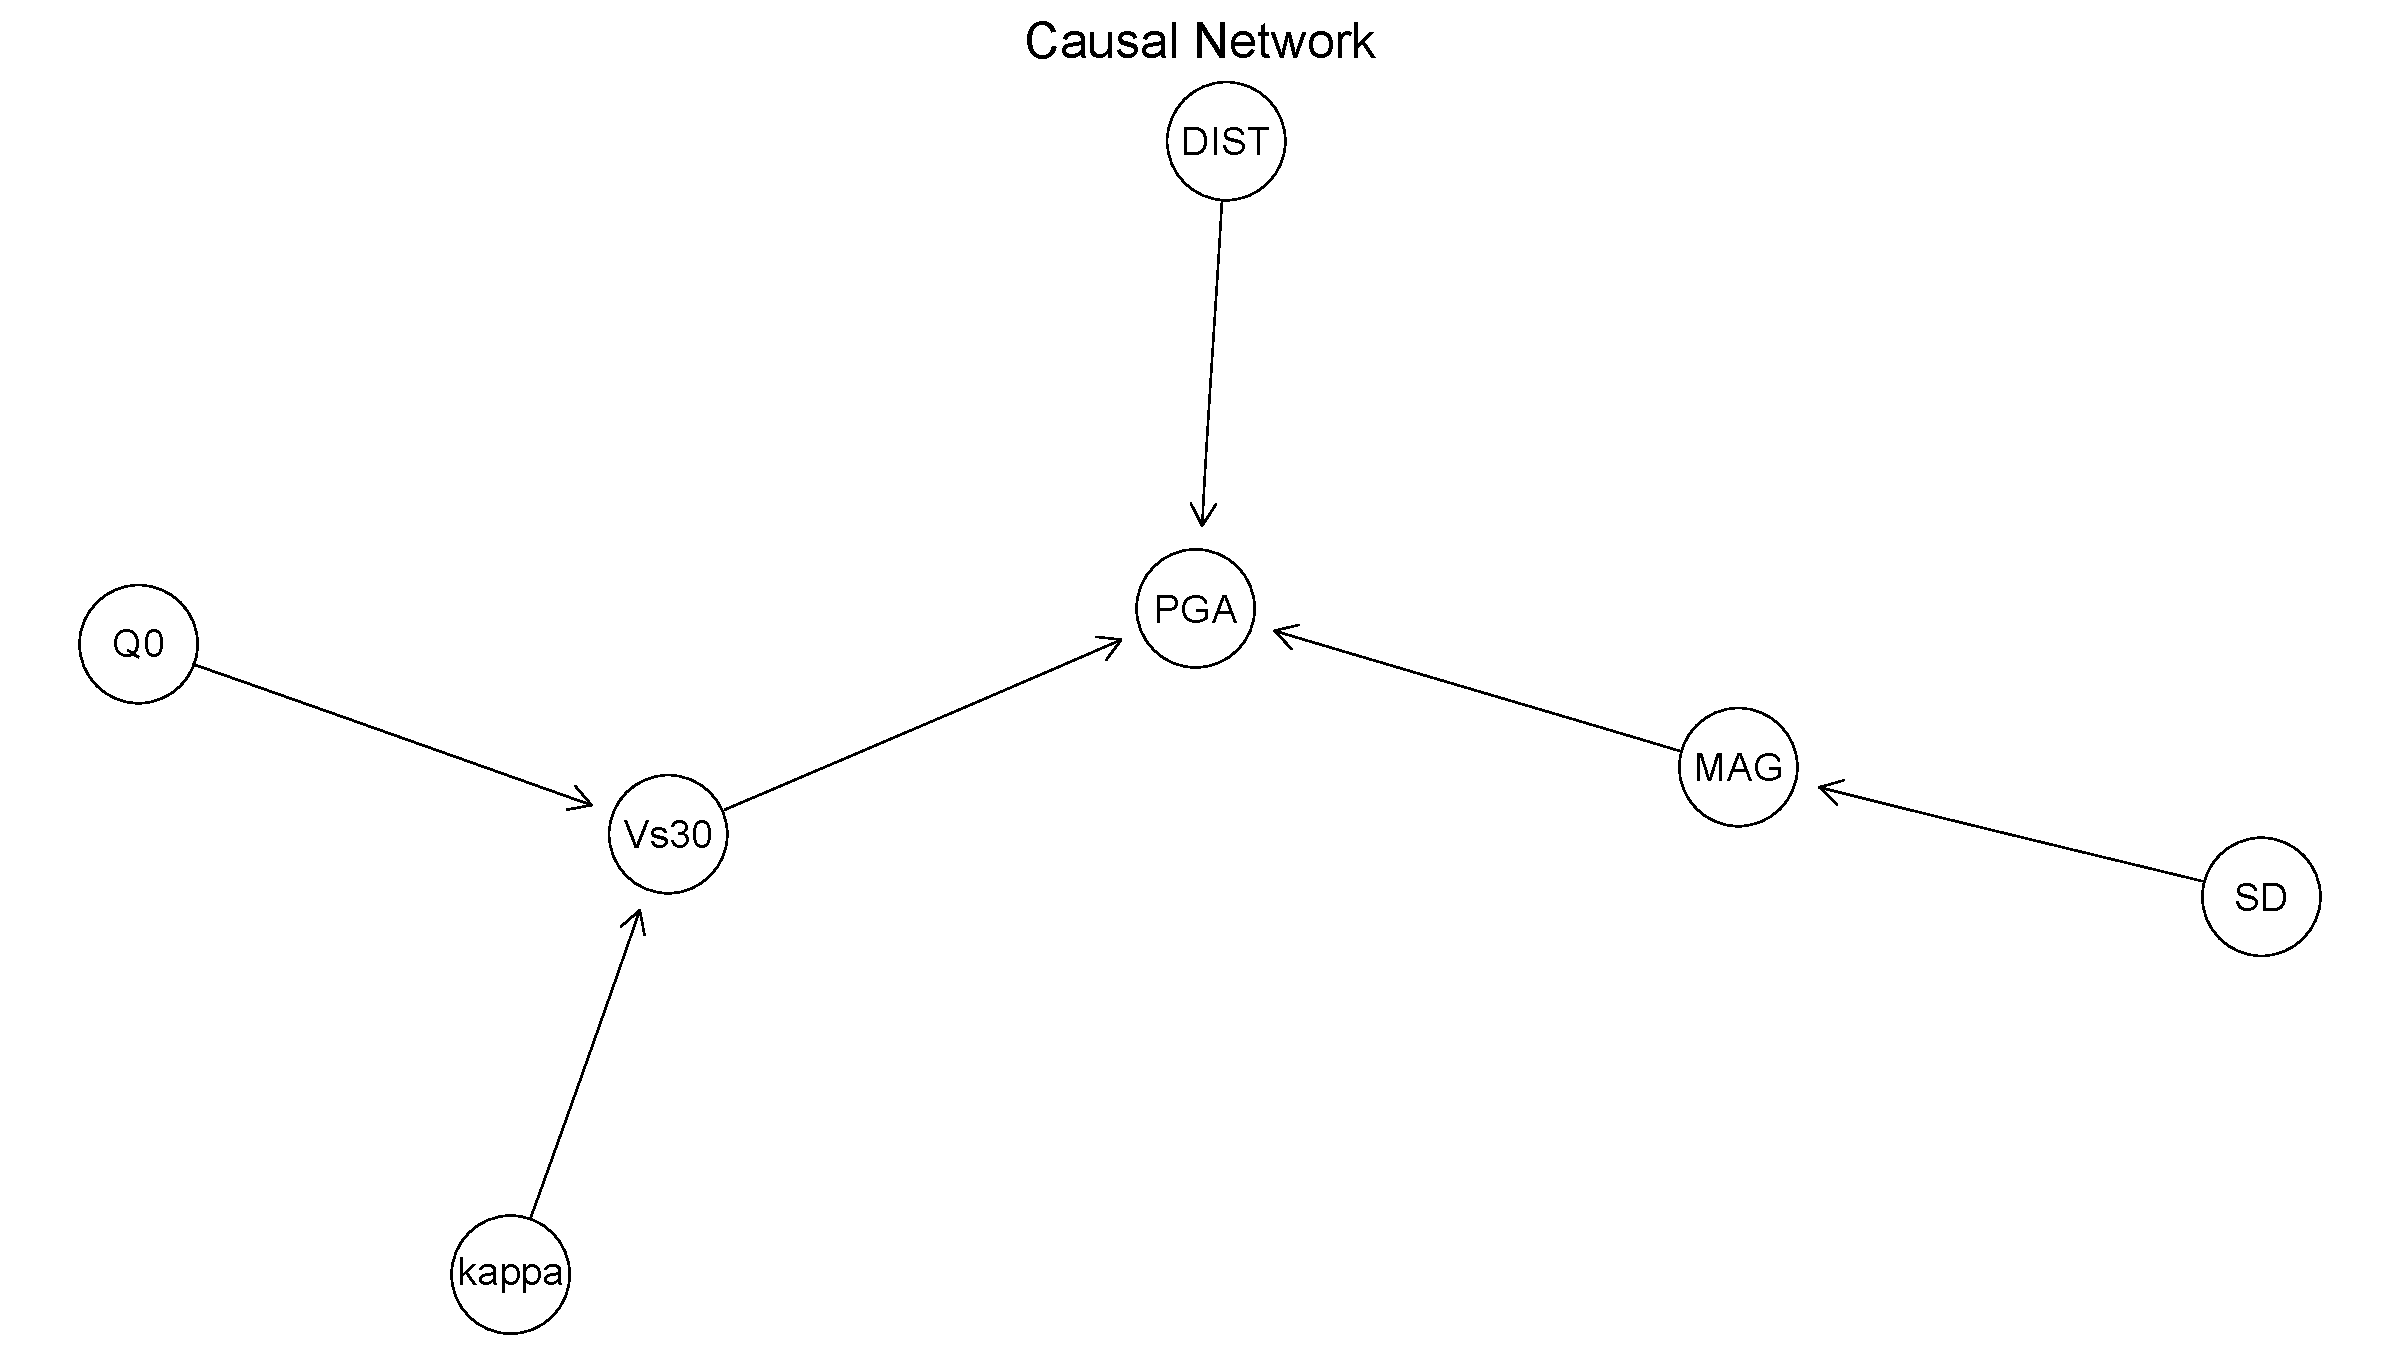
\includegraphics[scale=0.33]{Figures/causal.pdf}
		\rule{35em}{0.5pt}
	\caption[Causal Network]{A causal network representing the beliefs in dependency based on expert knowledge.}
	\label{fig:causal}
\end{figure}

One can argue that the attenuation behavior in deep layer (Q0) is independent from the one in shallow layers (kappa) because this difference reflects the varying materials and environment conditions. Nevertheless, since both are material properties, as well as the shear wave velocity in the first 30m ($V_s30$), one can imagine that their influence is mitigated by the shear wave velocity in the first 30m. The distance from the source (DIST) does not seem dependent on any other explanatory variable because one can argue having the same earthquake but choosing a different location on the earth's surface freely. Moment magnitude (MAG) and stress drop (SD) are dependent since they both refer to the energy that is released during an earthquake. Since the moment magnitude is proportional to the ruptured area the same value can be achieved by a wide range of possible combinations in the rupture's width and length. This is the reason why it is dependent on the stress drop, meaning one value of stress drop can have a distribution of moment magnitude values associated but not the other way around.
\footnote{After setting up the nets and running the computations, which took almost 2 weeks, I realized that this is not the best causal network I could design through my knowledge of the earthquake process. Q0 and kappa are attenuation parameters and only influence the amplitude of the seismic waves. It is questionable how this can have an influence on the seismic wave velocity. There also might be a dependency between the distance and the magnitude since larger earthquakes appear in greater depths and the distance employed in the Boore model is hypocentral distance and not epicentral. So this is more an example of a poorly designed causal net but changing this would have resulted in a re-computation.}\\
Another way to set up causal networks is to consult literature about the topic. In the case of Bayesian Networks for ground motion prediction sources could be \cite{kuehn2010} or \cite{Vogel2014}.\\

\subsection{The constraint-based Grow-Shrink Algorithm}

A third way of defining the structure of a Bayesian Network is to learn it from the data itself. Often, not all dependencies between the variables are known and human domain knowledge can also be misleading. So it is a natural extension to ask whether there are principled ways in the framework of Bayesian Networks to let also the structure come from the data. This can be done by extending the Bayesian paradigm so that the structure of a network becomes a random variable too. Now the task is to jointly estimate the parameters and the structure from the data. In the scope of this paper the constraint-based Grow-Shrink algorithm~\citep{margaritis2003} and the score-based Hill-Climber, using the Bayesian Information Criterion~\citep{schwarz} as score, are discussed.\\

Constraint-based algorithms perform independence tests between the random variables and then set up a network according to the found independencies. The task is one of finding the best minimal I-map. An I-map or independence map is a graph whose independence statements hold for the probability distribution among the variables. In the case where the graph captures all independence statements this is a perfect I-map. A minimal I-map is graph that is rendered not an I-map anymore by the removal of one edge. This is an important definition because the complete graph over a set of random variables is also an I-map but does not reveal any independencies and therefore carries parameters that are redundant. In practice not one single best minimal I-map is found but a class of graphs that carry the same independence statements and are therefore called I-equivalent~\citep{koller2009}. 
The Grow-Shrink algorithm tries to construct the structure of a network by finding the Markov Blankets of the variables. A Markov Blanket of one variable is a set of variables that renders that variable to be d-separated from all other variables. That means that knowing the state of any variable not in the Markov Blanket has no effect on knowing the state of the variable in interest. One could say that the Markov Blanket "shields" a variable from the influence of all other variables. Graphically, it is the set of parents, children and parents of the children of the variable in interest~\citep{koller2009}. In the growing phase of the Grow-Shrink algorithm independence tests between variables are performed which are the basis to decide whether a variable should be included in the Markov Blanket. These tests occur given the state of the Markov Blanket. Depending on the initial ordering of the variables this can lead to including redundant variables in the Markov Blanket which are subsequently removed by the independence test of the shrinking phase~\citep{margaritis2003}. In this assignment the mutual information (Equation~\ref{eqn:mutual}) is used as independence test.

\begin{equation}
I(X;Y) = \sum_{y \in Y} \sum_{x \in X} 
                 p(x,y) \log{ \left(\frac{p(x,y)}{p(x)\,p(y)}
                              \right) }, \,\! 
\label{eqn:mutual}
\end{equation}

It estimates the dependence between two variables by comparing the joint distribution to the product of the marginal distributions, since in the case of independence the joint distribution factorizes to the product of the marginal distributions. From a Venn-diagram point of view it calculates the area shared by two variables relative to the total area of the variables.\\
The learned network is visualized in Fig.\ref{fig:gs}. There are no direct dependencies between the explanatory variables. Even more, the variable $V_s30$ is completely ignored. By comparing this result to work of~\citep{Vogel2014},which uses a similar data set\footnote{ ;)}, one can find that this seems to be a consistent result when learning the structure of a Bayesian Network for ground motion prediction from data. One reason might be that $V_s30$ is merely a proxy in quantifying the capability of the soil to amplify the amplitudes of seismic waves.\\

\begin{figure}[htbp]
	\centering
		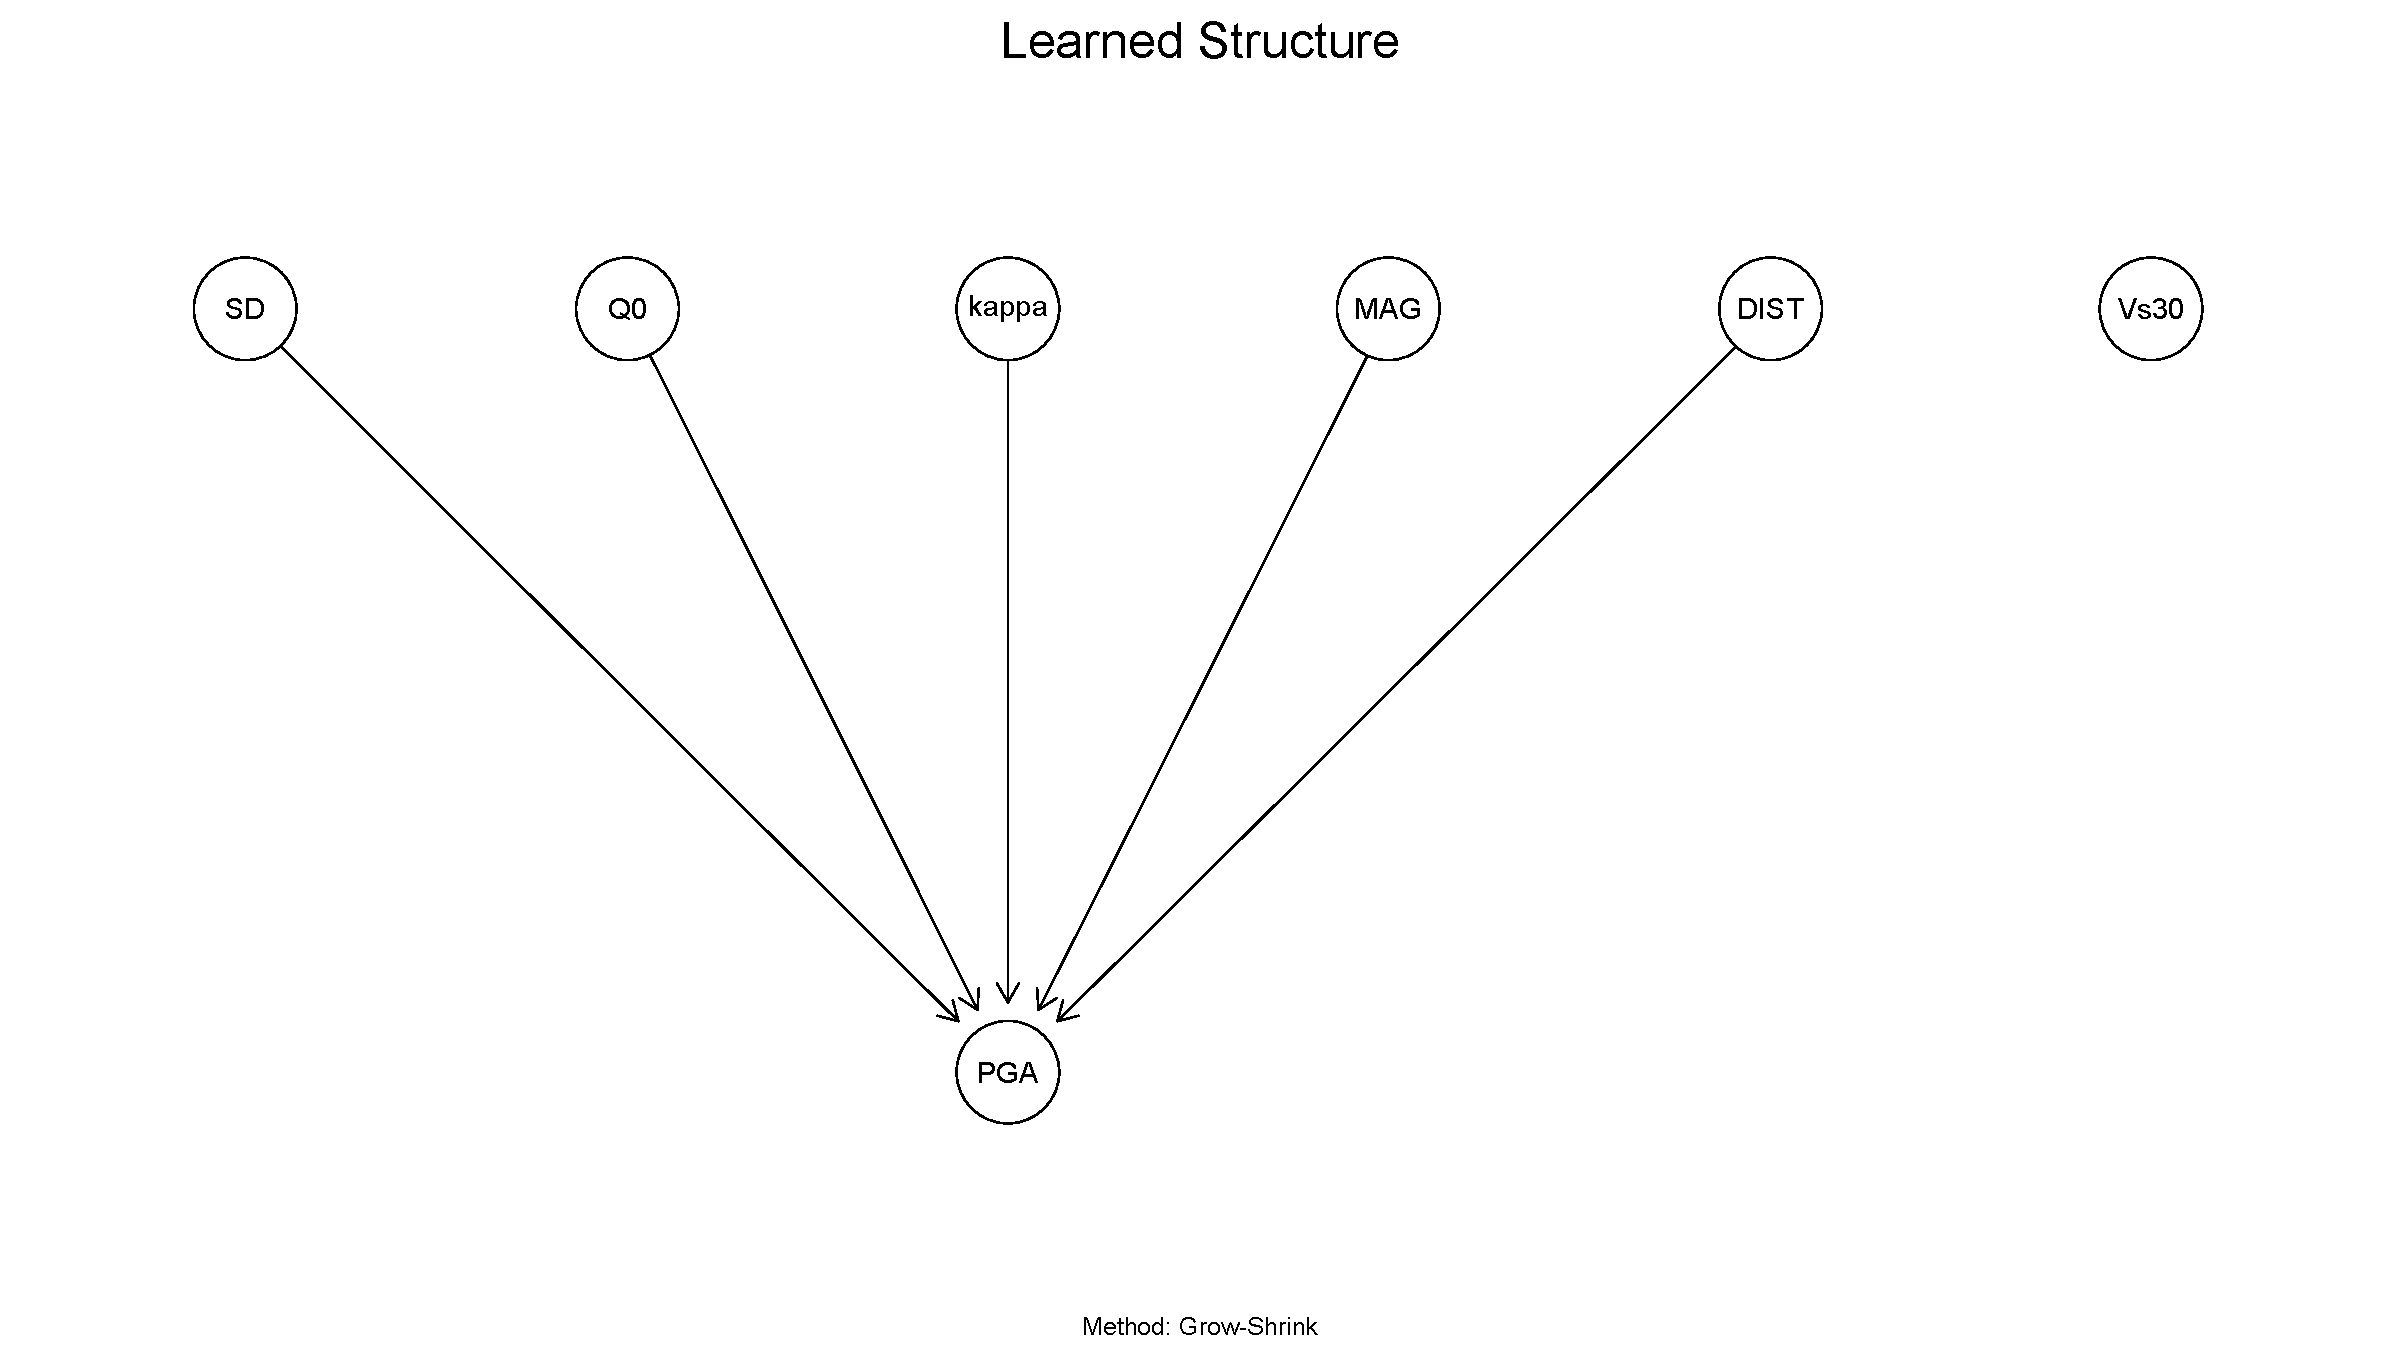
\includegraphics[scale=0.33]{Figures/gs_one.pdf}
		\rule{35em}{0.5pt}
	\caption[Contraint-based Grow-Shrink Network]{Bayesian Network constructed by the Grow-Shrink algorithm.}
	\label{fig:gs}
\end{figure}

\subsection{The score-based Hill-Climber Algorithm}

Score-based algorithms view the problem of finding the structure of a Bayesian Network from an optimization point of view. In contrast to the constraint-based algorithms, score-based ones do not try to construct the structure from information about single dependencies between variables, but take the network as a whole, compute a score and try to find the network that maximizes that score. Consequently, score-based algorithms pose a search problem in the space of possible network structures. Depending on the number of variables and the underlying probability distributions this is a NP-hard problem in most cases and requires some approximation techniques~\citep{koller2009}.\\
A Hill-Climber can be thought as the opposite of gradient descent since it tries to maximize a predefined score in contrast to minimizing an error term. For the construction of a Bayesian Network using the Hill-Climber algorithm a score consisting of the maximized likelihood L (Equation \ref{eqn:likelihood}), that gives the probability of the data being generated by the graph G and the parameters $\theta$, and the Bayesian Information Criterion (BIC) (Equation~\ref{eqn:BIC}~\citep{schwarz}) as a regularization term, consisting of the number of free parameters $k$ and the size of the data $n$, is used.

\begin{equation}
L = \operatorname*{arg\,max}_\theta P(x\mid \theta, G)
\label{eqn:likelihood}
\end{equation}

\begin{equation}
BIC = -2*ln L + k* ln(n)
\label{eqn:BIC}
\end{equation}


\begin{figure}[htbp]%
	\centering
		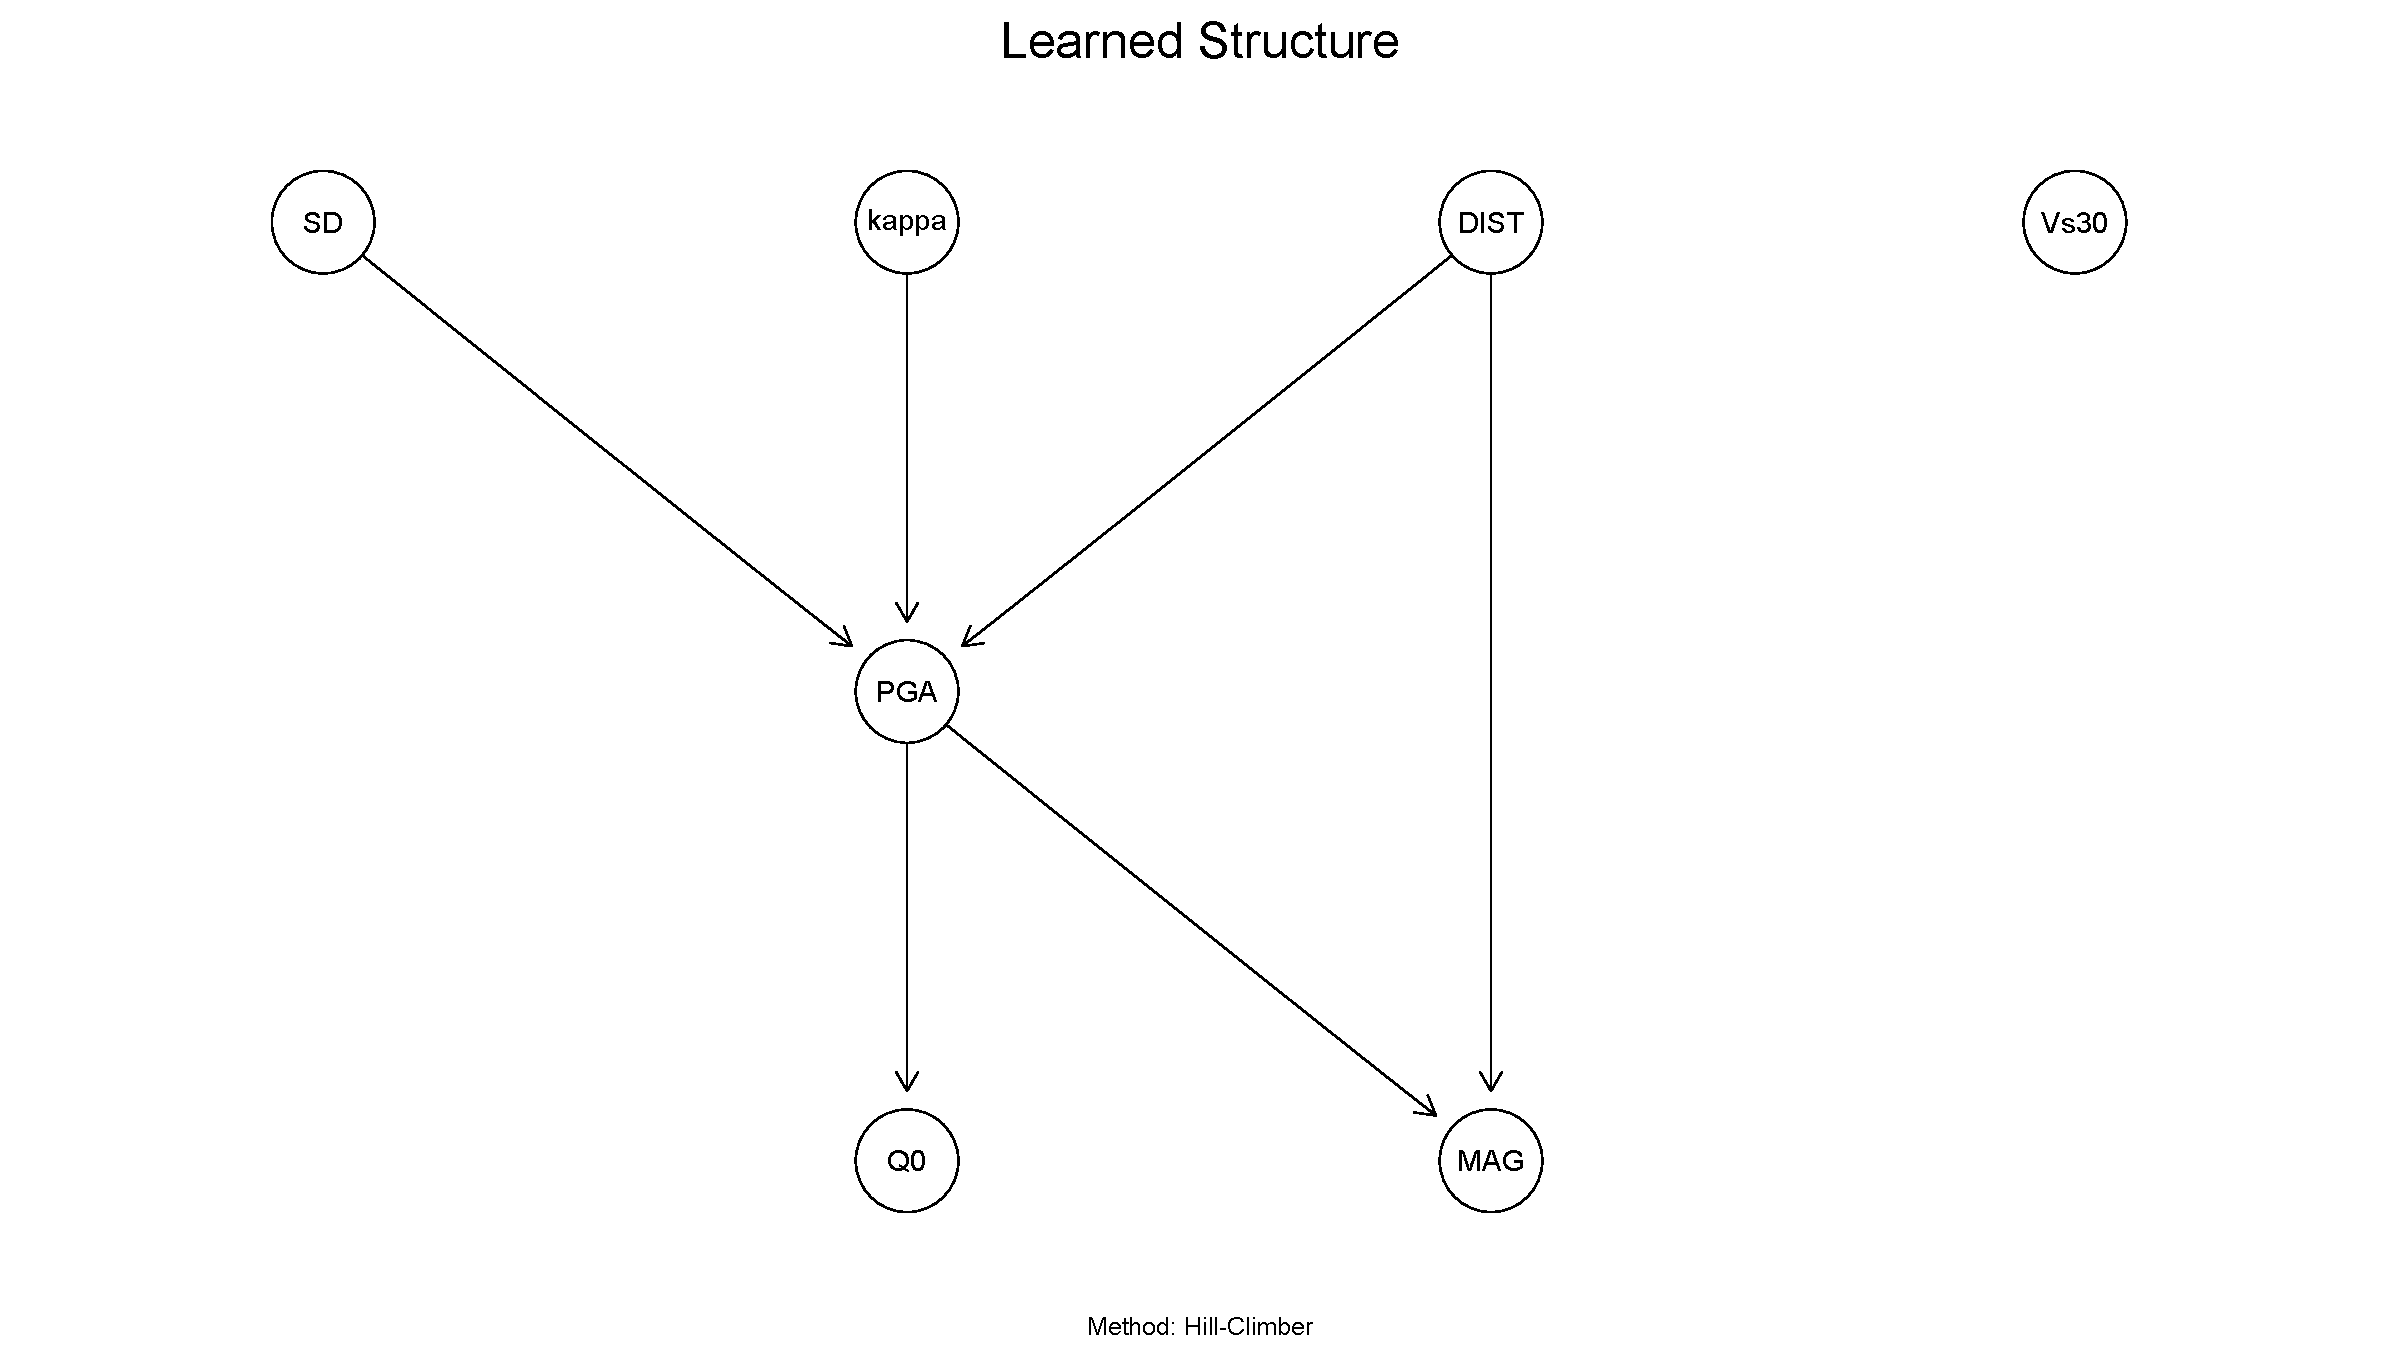
\includegraphics[scale=0.33]{Figures/hc_one.pdf}
		\rule{35em}{0.5pt}
	\caption[Score-based Hill-Climber Network]{Bayesian Network constructed by the Hill-Climber algorithm.}
	\label{fig:hc}
\end{figure}

The learned network from the Hill-Climber algorithm looks similar to the one learned by the Grow-Shrink algorithm. The only difference is a dependency between distance and moment magnitude. Since in the scope of this paper cross-validation is discussed, it should be noted that actually a series of networks was learned (Appendices~\ref{AppendixA1} and~\ref{AppendixA2}). Each of these networks is learned from a different set of data and besides the first fold of the Hill-Climber method the results for each method are consistent. This means that the structure of the learned network is not dependent on which data points are used to come up with the structure and it is a result that is expected by using synthetic data and learning the structure by random permutations of the data. 

%----------------------------------------------------------------------------------------

\section{Parameter Learning}

There are different ways to learn the associated parameters and therefore the probability distributions of a Bayesian Network. As noted before, because the model of~\cite{boore2003} has no simple analytic form and involves distributions from different families, the data has been discretized into intervals and discrete Bayesian Networks are learned using multinomial distributions.\\
In this assignment the parameters of the different networks have been learned using Bayes' Law. This is also called a maximum aposterior estimator (MAP) since the prior belief in the parameters are updated through the likelihood of the data been generated by a model with this parameters. With the posterior probability of the parameters being: 

\begin{equation*}
P(\theta\mid x) = \dfrac{P(x\mid \theta) P(\theta)}{P(x)}
\end{equation*}

the maximum aposteriori estimates of the parameters: 

\begin{equation*}
\theta_{MAP} = \operatorname*{arg\,max}_\theta~P(\theta\mid x)
\end{equation*}

Here, the structure of the Bayesian Network comes in handy because it simplifies the computations by making use of the independencies between variables. For each node in the network a probability table is calculated which depends only on the parent nodes and not on the full set of all variables. All the computations are performed with the bnlearn package for R~\citep{bnlearn}.
%----------------------------------------------------------------------------------------

